\documentclass[12pt,english,round]{article}
\usepackage[T1]{fontenc}
\usepackage[latin9]{inputenc}
\usepackage{geometry}
\geometry{verbose, tmargin=1in, bmargin=1in, lmargin=1in, rmargin=1in}
\usepackage{float}
\usepackage{booktabs}
\usepackage{amsmath}
\usepackage{amsthm}
\usepackage{amssymb}
\newtheorem{theorem}{Theorem}
\newtheorem{prop}{Prop}
\usepackage{graphicx}
\usepackage{setspace}
\usepackage{epstopdf}
\usepackage[section]{placeins}
\usepackage[toc,page]{appendix}
% \usepackage[authoryear]{natbib}
\usepackage[authoryear,longnamesfirst]{natbib}
\usepackage[colorinlistoftodos]{todonotes}
\usepackage{pdflscape}
\usepackage{rotfloat}
\usepackage{mathtools}
\doublespacing
\newcommand{\tinytodo}[2][]
{\todo[caption={#2}, size=\small, #1]{\renewcommand{\baselinestretch}{0.5}\selectfont#2\par}}
%\renewcommand{\abstractname}{\textsc{ABSTRACT}}
\makeatletter

\providecommand{\tabularnewline}{\\}
\usepackage{lscape}
\interfootnotelinepenalty=10000
\widowpenalty=10000
\clubpenalty=10000

%\usepackage{caption}
\usepackage{subcaption}

\makeatother

\begin{document}

\section{Exchange Rate Policy and Currency Excess Returns}


\begin{figure}[htp!]
    \centering
    \caption{Interest Rate Differential (Resid.)}
    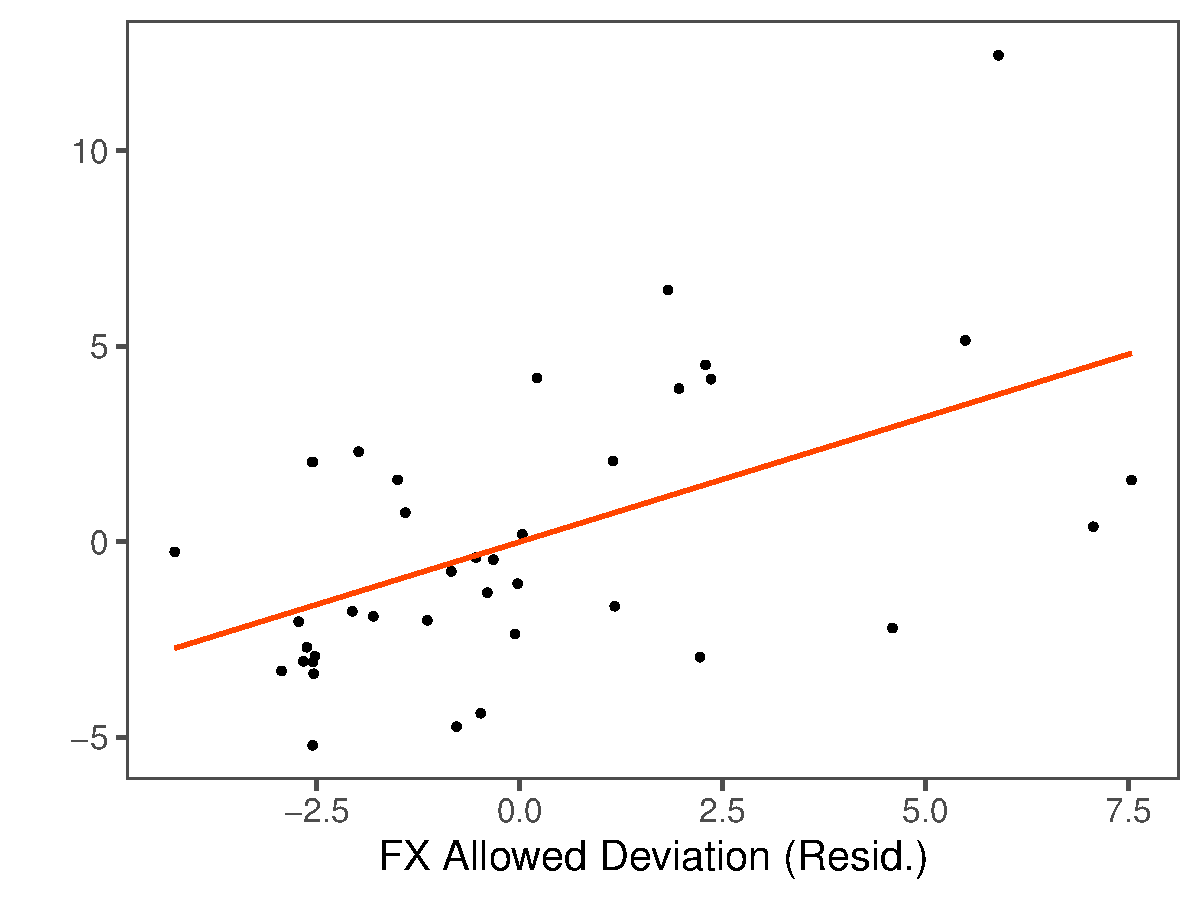
\includegraphics[width=0.66\textwidth]{Figure_FP_ERA.pdf}
\end{figure}

\vspace{1em}

\begin{table}[htp]
\begin{center}
\caption{Interest Rate Differential}
\begin{tabular}{l c c c }
\hline
 & (1) & (2) & (3) \\
\hline
Country Size            & $-12.91^{**}$ &             & $-28.12^{***}$ \\
                        & $(5.08)$      &             & $(9.20)$       \\
Allowed FX Dev.         &               & $0.34$      & $0.64^{**}$    \\
                        &               & $(0.24)$    & $(0.24)$       \\
\hline
Num. obs.               & 39            & 39          & 39             \\
R$^2$                   & 0.06          & 0.10        & 0.32           \\
\hline
\multicolumn{4}{l}{\scriptsize{$^{***}p<0.01$, $^{**}p<0.05$, $^*p<0.1$}}
\end{tabular}
\end{center}
\end{table}


\clearpage

\begin{figure}[htp!]
    \centering
    \caption{Currency Excess Returns (Resid.)}
    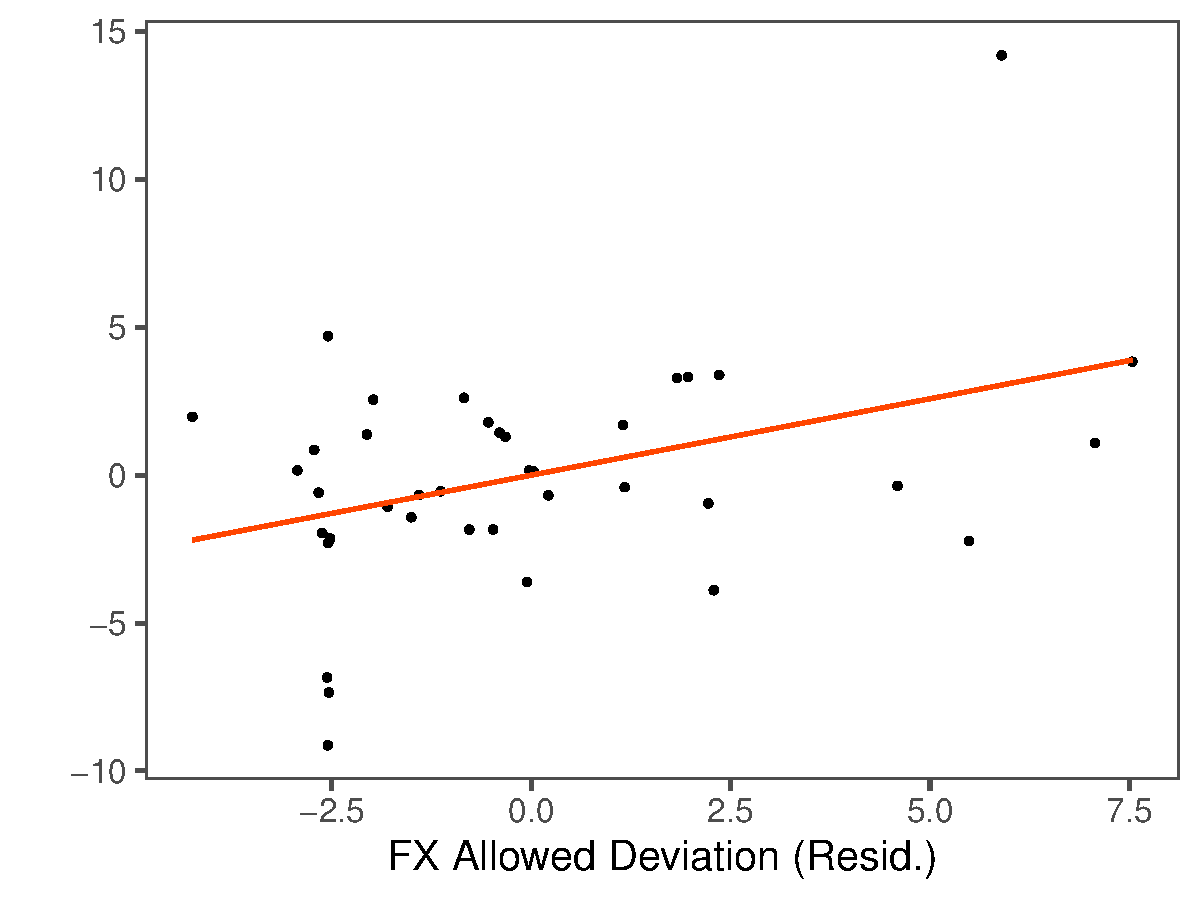
\includegraphics[width=0.66\textwidth]{Figure_RX_ERA.pdf}
\end{figure}

\vspace{1em}


\begin{table}[htp]
\begin{center}
\caption{Currency Excess Returns}
\begin{tabular}{l c c c }
\hline
 & (1) & (2) & (3) \\
\hline
Country Size            & $-1.90$      &          & $-14.17^{*}$ \\
                        & $(4.26)$     &          & $(8.38)$     \\
Allowed FX Dev.         &              & $0.37$   & $0.52^{*}$   \\
                        &              & $(0.22)$ & $(0.28)$     \\
\hline
Num. obs.               & 39           & 39       & 39           \\
R$^2$                   & 0.00         & 0.11     & 0.16         \\
\hline
\multicolumn{4}{l}{\scriptsize{$^{***}p<0.01$, $^{**}p<0.05$, $^*p<0.1$}}
\end{tabular}
\end{center}
\end{table}

\clearpage

\begin{figure}[htp!]
    \centering
    \caption{Capital Intensity (Resid.)}
    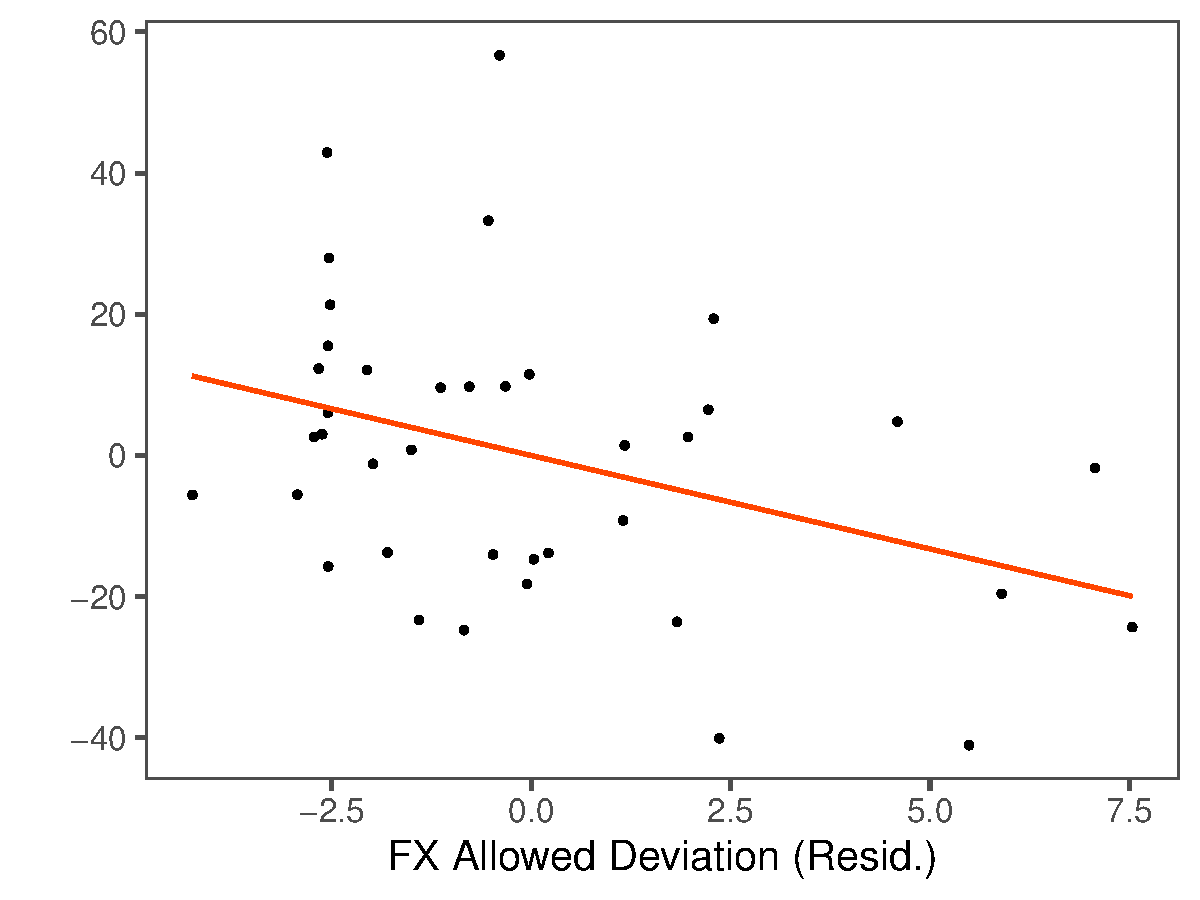
\includegraphics[width=0.66\textwidth]{Figure_KY_ERA.pdf}
\end{figure}

\vspace{1em}

\begin{table}[htp]
\begin{center}
\caption{Capital Intensity}
\begin{tabular}{l c c c }
\hline
 & (1) & (2) & (3) \\
\hline
Country Size            & $32.65$        &                & $95.55^{***}$  \\
                        & $(20.64)$      &                & $(30.94)$      \\
Allowed FX Dev.         &                & $-1.63^{*}$    & $-2.65^{***}$  \\
                        &                & $(0.95)$       & $(0.93)$       \\
\hline
Num. obs.               & 39             & 39             & 39             \\
R$^2$                   & 0.01           & 0.07           & 0.15           \\
\hline
\multicolumn{4}{l}{\scriptsize{$^{***}p<0.01$, $^{**}p<0.05$, $^*p<0.1$}}
\end{tabular}
\end{center}
\end{table}

\clearpage

\section{Capital Intensity and Currency Excess Returns}

\begin{figure}[htp!]
    \centering
    \caption{Capital Intensity}
    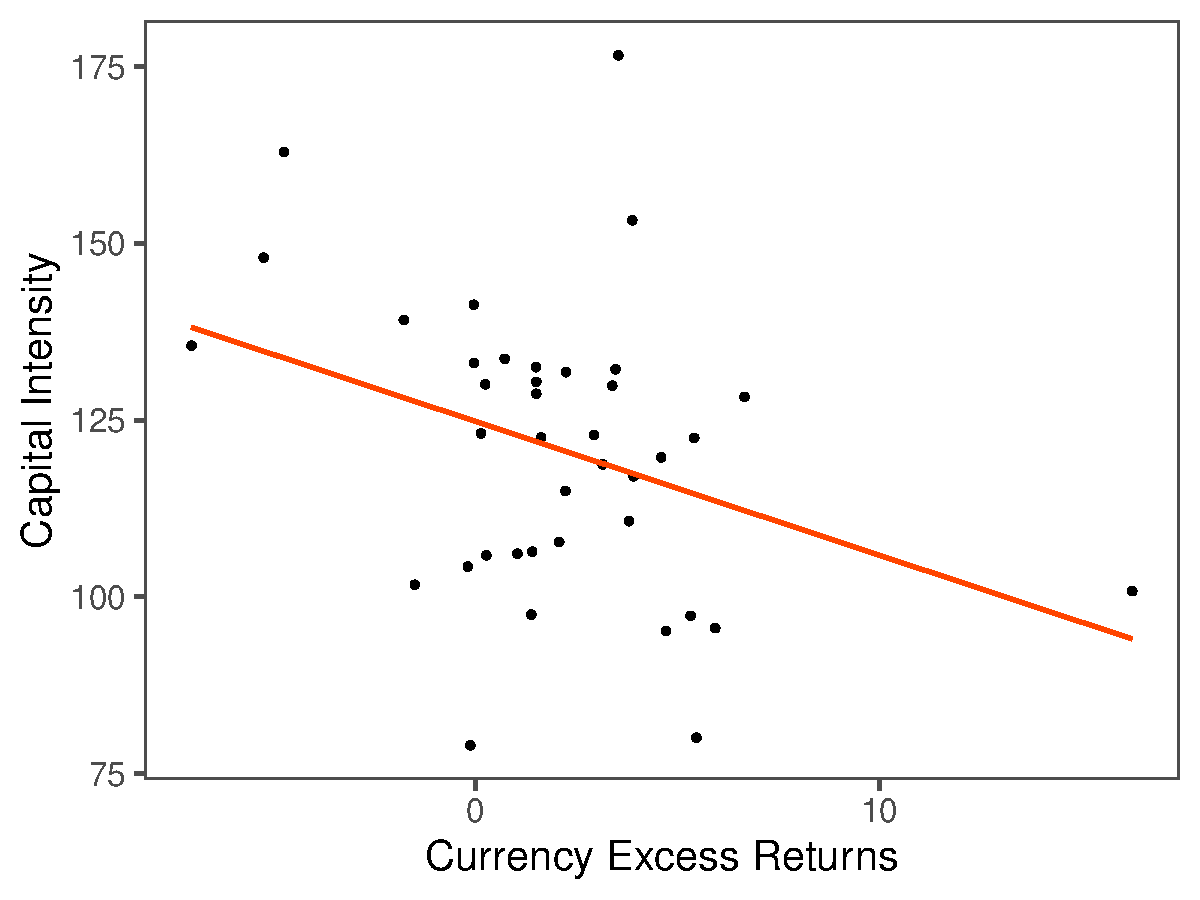
\includegraphics[width=0.66\textwidth]{Figure_RX_KY.pdf}
\end{figure}


\begin{table}[htp]
\begin{center}
\caption{Capital Intensity}
\begin{tabular}{l c }
\hline
 & (1) \\
\hline
Currency Excess Returns & $-1.89^{***}$  \\
                        & $(0.67)$       \\
\hline
Num. obs.               & 39             \\
R$^2$                   & 0.12           \\
\hline
\multicolumn{2}{l}{\scriptsize{$^{***}p<0.01$, $^{**}p<0.05$, $^*p<0.1$}}
\end{tabular}
\end{center}
\end{table}




\end{document}
